\section{Network of ``Parameterization Prediction"}
\subsection{Problem and Notations}
The specific problem is how to reconstruct a complete 3D shape of an object with a single 2D image as reference. 
\subsection{Network overview}
\begin{figure}[htbp]
	\centering
	\includegraphics[width=\linewidth]{img/net/overview}
	\caption{The overview of the network}
	\label{fig:overview}
\end{figure}
\subsection{K-neighbor Point Net for Surface Mapping}
When a potter crafting something from a lump of clay, she do it by applying a serious of squeeze. Each squeeze only affect the clay locally, but all the squeeze together turn the clay into graceful shape. Our shape generation network is designed by stimulating such process. We employ a simpler version of PointNet\cite{PointNet} that is a network forged with the symmetric functions and apply it on each k-neighbor of input point set to predict a drift for the center of these k-neighborhoods. We do this deformation. Figure~\ref{fig:knpointnet} shows the detailed structure of this build block. 
We this 
\begin{figure}[htbp]
	\centering
	\includegraphics[width=\linewidth]{img/net/k-n_pointnet}
	\caption{The structure of K-neighbor Point Net}
	\label{fig:knpointnet}
\end{figure}

\subsection{Convolution Network for Semantic Analysis}


